\chapter{Aplicaciones del Análisis de Intervalos a las superficies implícitas}

Como ya hemos explicado en el capítulo anterior, el Análisis de Intervalos es una herramienta bastante fiable con respecto a los problemas de redondeo de los ordenadores. Además tiene aplicaciones en muchas áreas como:
\begin{itemize}
	\item Gráficas por ordenador.
	\item Detección de colisiones.
	\item Errores de aproximación en la transferencia de datos entre sistemas CAD/CAM.
	\item Ray Tracing de superficies paramétricas.
	\item Ray Tracing de superficies implícitas.
\end{itemize}

El Análisis de Intervalos ha sido usado en Infografía en especial para la creación de algoritmos de subdivisión fidedignos. Estos algoritmos pueden evaluar áreas o espacio para detectar la{ \em existencia} de superficies o curvas. Esto permite la creación de estructuras como árboles octales o cuaternarios, octrees y quadtrees en inglés de forma respectiva.

Este capítulo comienza con la introducción de diferentes algoritmos de subdivisión de intervalos. A continuación presentamos diferentes técnicas para desarrollar Ray Tracing, centrándonos en las basadas en Aritmética de Intervalos. Finalmente se incluye una comparación entre aproximaciones basadas en intervalos para encontrar las raíces de las intersecciones para conocer la eficiencia.

\section{Algoritmos de subdivisión recursiva}

Existen infinidad de técnicas para representar objetos geométricos como representaciones poligonales, técnicas de subdivisión espaciales, parches paramétricos... El proceso de visualización mediante Análisis de Intervalos conbina características de de todos las técnicas nombradas, aunque la más común suele ser la subdivisión del espacio. Éste es usado para representar objetos geométricamente  y luego aplicar estrategias de renderizado como el Ray Tracing.

Los métodos de subdivisión del espacio tienen como propósito{ \em encerrar} al objeto.  Esto es, por ejemplo en el método de los árboles octales, si una región cúbica encierra un objeto entonces podemos dividir el cubo en ocho octantes iguales. Cada nuevo cubo, u octante, es evaluado para asegurarnos que contiene alguna parte del objeto. Este proceso continua hasta un nivel predefinido de subdivisión.
\\Este proceso crea una estructura octal con información sobre el objeto que puede ser utilizada para crear una visualización directa o acelerar otras técnicas de visualización.

\subsection{Subdivisión espacial usando Aritmética de Intervalos}

El algoritmo de a subdivisión se basa en la subdivisión recursiva del espacio que contiene al objeto para generar ocho cubos llamados octantes.

Un octante consiste en una región cúbica definida por tres intervalos, en el que cada uno de ellos representa los valores de frontera del octante en cada una de las dimensiones. Los octantes que no contienen ningún punto de la superficie son descartados.

Este proceso permite la creación de estructuras que describan el objeto de forma geométrica. La creación de estructuras como los árboles octales es directa. Un árbol octal es un tipo de estructura  que representa el espacio ocupado por varios objetos en una escena tridimensional. La versión bidimensional es llamado árbol cuaternario.

En conclusión estamos ante un tipo de árbol en el que cada nodo representa regiones y sus hojas son regiones aún más pequeñas que contienen parte de los objetos

Es posible usar este algoritmo para representar operaciones entre diferentes funciones implícitas. Por ejemplo, Suffern et al.\cite{Suffern03} introdujo una técnica para renderizar la intersección entre dos superficies implícitas basada en un árbol octal. Esta técnica usaba Aritmética de Intervalos para descartar regiones que no contenían alguna de ambas superficies. Si la región contiene a ambas superficies se subdivide y se repite el mismo análisis.

Los octantes que contienen alguna parte de la superficie se subdividen en otras ocho regiones que se evalúan para saber si siguen conteniendo alguna parte de la superficie.

Dada una superficie implícita, definida por $f(x,y,z) = 0$, y una región cúbica definida por tres intervalos $X$, $Y$ y $Z$. Usaremos la extensión unida de $f$ definida en el capítulo anterior para saber si la superficie interseca a la región cúbica. A esta extensión la denotaremos por $F(X,Y,Z)$.

El algoritmo funciona como sigue: Si $0 \in F(X,Y,Z)$ significa que la región interseca a al superficie, en caso contrario, la región puede descartarse.

Las regiones del espacio que contienen parte de la superficie se subdividen de forma recursiva y se evalúan de nuevo hasta que alcanzamos el tamaño de mallado deseado, el cual habremos seleccionado en base a la resolución que necesitemos. Al final del algoritmo tendremos una lista de cubos que contienen partes de la superficie, pero parte de esos cubos contendrán regiones que no son solución a nuestro problema. El algoritmo de subdivisión usando funciones inclusión sería el siguiente:
\begin{verbatim}
Evaluate(X,Y,Z):
   If(0 belongs to F(X,Y,Z))
      If(X or Y or Z <= Threshold)
         Add (X,Y,Z) to solution list
      Else
         Subdivide X into X_1 and X_2
         Subdivide Y into Y_1 and Y_2
         Subdivide Z into Z_1 and Z_2
         Evaluate (X_i,Y_j,Z_k) for i,j,k in {1,2}
   Else
      The octant is rejected
\end{verbatim}

Este algoritmo tiene muchas debilidades. La principal es que el algoritmo es muy dependiente del número de subdivisiones requeridas para alcanzar la resolución deseada, lo que provoca un gran coste computacional.

Aunque este algoritmo es muy útil en el caso tridimensional se puede usar para casos bidimensionales e incluso para rasterizar curvas algebraicas, véase \cite{Oliveira00,Taubin94}.

\subsection{Mejorando el proceso de subdivisión}

Existen muchas técnicas para mejorar el proceso de subdivisión. El principal objetivo de tales técnicas es permitir el diseño de algoritmos de subdivisión más eficientes y robustos.

Una versión adaptativa del algoritmo trabaja con la curvatura de la superficie durante el propio proceso de subdivisión. Balsys et al. \cite{Balsys01} desarrollaron un algoritmo adaptativo para mejorar la creación de la estructura del árbol octal. Esto soluciona los problemas surgidos por la diferencias de profundidad entre nodos adyacentes.

En \cite{Oliveira00,Suffern03} las técnicas adaptativas se usan para garantizar que las subdivisiones son lo suficientemente pequeñas como para contener partes de una curva con una curvatura relativamente grande. Esto se consigue evaluando el gradiente de la curva en cada subdivisión: un gradiente muy grande significa que la curva varía mucho dentro de la región en la que estamos trabajando. Por tanto tenemos que generar cubos pequeños para representar la curvatura.

Carvalho et al.\cite{Carvalho98} proporcionó ciertas condiciones para detener el proceso de subdivisión recursiva cuando las celdas son lo suficientemente pequeñas y no contienen intersecciones cerradas de la curva.

Bühler\cite{Buhler02} desarrolló una estimación lineal implícita basada en intervalos, ILIE por su siglas en inglés, que consiste en un cierre lineal de un objeto adaptado a la topología intrínseca del mismo. Cada celda se reduce a partes que sólo contienen la correspondiente ILIE, lo que reduce el número de subdivisiones del proceso total. Esto, por supuesto, reduce el tiempo de computación.

Standder y Hart\cite{Stander97} nos muestran cómo los puntos críticos de la función afectan a la topología de la superficie implícita. Usaron la Aritmética de Intervalos para encontrar tales puntos y, tras esto, modificaron la poligonalización para acomodarla a los cambios topológicos.

Duff\cite{Duff92} desarrolló una aplicación geométrica de los intervalos usando árboles en donde las hojas son funciones implícitas. El algoritmo tiene en cuenta la información del árbol completo en cada subdivisión, obteniendo así una escena completa con varios objetos correctamente renderizados en la misma escena.

\section{Ray Tracing eficiente aplicado a superficies implícitas}

En esta sección abarcaremos distintas mejoras desarrolladas por distintos autores para realizar un Ray Tracing eficiente en superficies implícitas. Estos trabajos se centran en la creación de intersecciones fidedignas. Los autores aplican distintas técnicas numéricas para controlar la pérdida de raíces debido al uso de algoritmos basados en números de coma flotante. Esto puede generar que ciertas partes de las superficies más{ \em finas} puedan perderse durante el proceso de renderización. Aunque este tipo de superficies son casos especiales  sería deseable obtener un método que también fuera capaz de cubrir estos casos.

Otro problema relacionado con el Ray Tracing  es la eficiencia de los algoritmos. Whitted\cite{Whitted80} menciona que el 95 por ciento del gasto de tiempo de renderizado era debido a las intersecciones en escenas complejas. El Ray Tracing es lento debido a que necesita de muchas intersecciones para cada píxel. Esto se incrementa en las superficies implícitas e incluso más con la Aritmética de Intervalos.

\subsection{Aproximación por muestreo puntual}

Los test de intersección se pueden desarrollar en dos pasos:
\begin{enumerate}
\item Encontrar la raíz, en donde el primer intervalo que la contiene es seleccionado.
\item Refinamiento de la raíz, en donde el intervalo que la contiene se reduce hasta llegar a un tamaño prefijado.
\end{enumerate}

La clave en el primer paso es garantizar que el intervalo contiene una única raíz de la función implícita. Este paso normalmente es más complicado y puede resolverse con métodos como el de la bisección. Sin embargo, este método puede causar problemas como la convergencia a la raíz equivocada o, directamente, la no convergencia.
\begin{verbatim}
Bisection(t_1,t_2):
   t_m = (t_1 + t_2)/2   
   If(f(t_m) == 0)
      t_m is a root
   Else
      If(abs(t_2 - t_1) < Threshold)
         There are no roots
      Elif(f(t_1)*f(t_m) < 0)
         Bisection(t_1,t_m)
      Else
         Bisection(t_m,t_2)
\end{verbatim}

Una alternativa al método de la bisección es el método de Newton, el cual tiene la ventaja de que, en caso de converger, lo hace de forma cuadrática en lugar de lineal como el método de la bisección. Sin embargo, el método de Newton puede no converger a ninguna de las raíces o, en algunos casos, divergir\cite{Hart01}.

Un ejemplo de los problemas del muestreo puntual es el de la imagen \ref{florez45}. Si los intervalos iniciales son demasiado grandes, imagen a), se pierde mucha información y, por tanto, raíces. Si usamos un tamaño más pequeño de intervalos el problema no se resuelve del todo, como se puede ver en b). Además, intervalos pequeños significan pérdida de eficiencia. El problema se soluciona usando Aritmética de Intervalos, casos c) y d). Incluso usando una precisión pequeña en el método de la bisección, caso c), el resultado es mejor que en los anteriores. El mejor resultado posible sería el d) que es cuando el método de la bisección alcanza la precisión de máquina.
\begin{figure}[h]
	\centering
	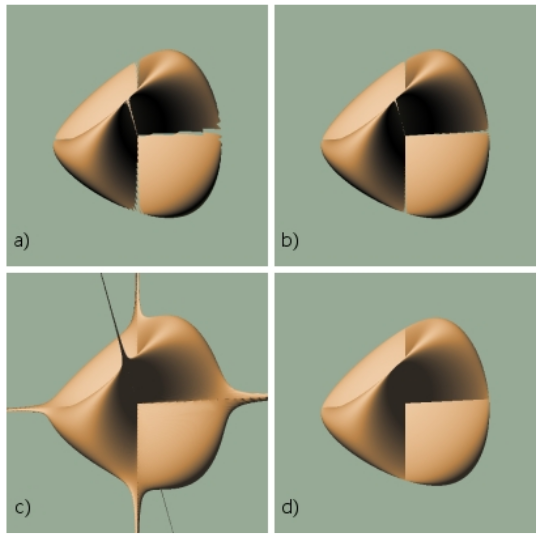
\includegraphics[scale=0.5]{images/florez5.png}
	\caption{Imágenes obtenidas por muestreo puntual. a) Sin Aritmética de Intervalos e intervalo de tamaño 0.001. b) Sin Aritmética de Intervalos e intervalo de tamaño 0.0001. c) Con Aritmética de Intervalos y bisección con precisión 0.0001. d) Con Aritmética de Intervalos y bisección con precisión máquina.}
	\label{florez45}
\end{figure}

\subsection{Aproximación por Aritmética de Intervalos}

Mitchell\cite{Mitchell90} propuso el uso de Aritmética de Intervalos para encontrar la raíz de una forma segura. La extensión unida de la función intersección $f$ es
\begin{equation}
F(T) = f(c_x + T(x_s - c_x), c_y + T(y_s - c_y), c_z + T(y_z - c_z)).
\nonumber
\end{equation}
Los valores $c_x$, $c_y$ y $c_z$ indica el punto de vista del observador y los valores $x_s$, $y_s$ y $z_s$ indican el punto donde el rayo interseca la pantalla y $T$ es el parámetro del intervalo. La diferencia con la definición clásica es el uso del parámetro del intervalo $T$, que toma intervalos como valores en lugar de puntos reales.

La ecuación anterior se conoce por{ \em función inclusión} para la superficie implícita. Esta función puede ser evaluada usando cualquier intervalo de $T$. Si el resultado de la evaluación es $0 \notin F(T)$ podemos asegurar que no hay ninguna raíz de $f$ en el valor actual de $T$. Aún así esta función no consigue el resultado contrario, esto es, para conocer si existen raíces para cada valor de $T$. Esto es debido a que en cada operación los límites del intervalo se redondean al alza y a la baja para garantizar que cualquier resultado posible no se pierda. Este redondeo incluye valores que no son parte de la evaluación de la función, por ello el cero puede ser incluido mediante cualquiera de las operaciones de redondeo. Por tanto, la función inclusión se usa como función descarte. 

Para saber si hay una única raíz en el intervalo usamos la extensión unida $F'$ de la derivada $f'$. El algoritmo propuesto por Mitchell es el siguiente:
\begin{verbatim}
Mitchell(T as [t_1,t_2]):
   If(0 not in F(T))
      If()
         If(f(t_1)*f(t_2) <= 0)
            Root refinement over T using Bisection or Newthon method
      Else
         T_1 = [t_1,(t_1 + t_2)/2]
         T_2 = [(t_1 + t_2)/2,t_1]
         
         If(width(T_1) >= threshold)
            Mitchell(T_1)
         Else
            Root refinement over T_1 using Bisection or Newthon method
         
         If(width(T_2) >= threshold)
            Mitchell(T_2)
         Else
            Root refinement over T_2 using Bisection or Newthon method
   Else
      Reject T
\end{verbatim}

El algoritmo comienza evaluando el intervalo $T$ usando la función inclusión. En el caso de que el cero esté contenido en el resultado, la derivada de la función implícita es se evalúa usando el valor del intervalo de $T$. Si el cero no pertenece al resultado de la evaluación de la derivada se comprueba que los valores de los extremos del intervalo sean de signo contrario y, en caso de darse, sabemos que sólo hay una sola raíz en el intervalo $T$. Por tanto podríamos realizar el proceso de refinamiento del intervalo.
\\En el caso de que al evaluar la función inclusión y la derivada el cero esté contenido, subdividimos el intervalo $T$ en dos y repetimos el proceso con los nuevos intervalos.

Otra consideración a tener en cuenta es la anchura que a la que los intervalos pueden llegar a alcanzar antes de finalizar la búsqueda de la raíz y comenzar el refinamiento del intervalo. Por ejemplo, cuando las raíces se encuentran en la tangente, la convergencia será siempre hacia estas raíces. En tal caso, la derivada es siempre cero y el proceso siempre termina cuando se alcanza un valor mínimo de anchura.

En otros casos no hay garantía de que el mínimo de anchura permitido contenga alguna raíz. En tal caso se puede establecer el mínimo en la precisión del ordenador, lo que incrementa significativamente las probabilidades de que contenga una raíz\cite{Capriani00}.

Mitchell no usó redondeo en sus operaciones entre intervalos. Consideraba que el uso de coma flotante en la aritmética proporcionaba suficiente precisión para la renderización de las superficies. La razón que esgrimía era que la Aritmética de Intervalos era que aumentaba el tiempo de renderización.

Finalmente, este algoritmo propone resolver el refinamiento del intervalo usando técnicas clásicas como ĺos métodos de bisección, Newton o cualquier otro suficientemente rápido para renderizar las superficies. Esto es debido a que, según Mitchell, La Aritmética de Intervalos es demasiado lenta para realizar este proceso.

\subsection{Mejorando la aproximación por Aritmética de Intervalos}

Si el algoritmo para encontrar la raíz se desarrolla usando la bisección clásica de intervalos, mismo algoritmo que en la sección anterior pero sin la verificación de la derivada, la eficiencia del algoritmo puede bajar drásticamente.

Capriani et al. \cite{Capriani00} nos muestran que hay algoritmos basados en intervalos para encontrar raíces eficaces y suficientemente rápidos como para renderizar una superficie implícita.
\begin{verbatim}
Newton(T as [t_1,t_2]):
   If(0 in F(T))
      If(0 not in F'(T))
         t_m = t_1 + midpoint(T)
         NT = t_m - f(t_m)/F'(T)
         NTT = NT intersecting with T
        
         If(NTT is empty)
            There's no root
         Else
            Newton(NTT)
        
      Else
         T_1 = [t_1,midpoint(T)]
         T_2 = [midpoint(T), t_2]
         
         If(width(T_1) >= Threshold)
            Newton(T_1)
         Else
            T_1 is the root
            
         If(width(T_2) >= Threshold)
            Newton(T_2)
         Else
            T_2 is the root
   Else
      Reject T
\end{verbatim}

El método de intervalos de Newton es una aproximación muy buena que es más rápida que la versión clásica de la bisección. El método de intervalos de Newton tiene a menudo convergencia cuadrática, pero requiere del cálculo de las derivadas.

Capriani et al. propusieron una importante mejora del método mediante un operador Alefeld-Hansen. El operador es obtenido cuando $0 \in F'(T)$. Si $T = [t_1,t_2]$ se define
\begin{equation}
\frac{1}{F'(T)} = \left\{ \begin{tabular}{l l l}
$\left[ \frac{1}{t_2}, \infty \right]$ & & si $t_1 = 0$, \\ \\
$\left[ - \infty, \frac{1}{t_1} \right]$ & & si $t_2 = 0$, \\ \\
$\left[ - \infty, \frac{1}{t_1} \right] \cup \left[ \frac{1}{t_2}, \infty \right]$ & & Cualquier otro caso.
\end{tabular}
\right.
\nonumber
\end{equation}
Véase \cite{Alefeld70,Hansen78}.

Usando aritmética extendida\cite{Hansen03} el operador es
\begin{equation}
AH(T) = \left[ midpoint(T) - \frac{f(midpoint(T))}{F'(T)} \right] \cap T.
\nonumber
\end{equation}

El operador de Alefeld-Hansen se puede añadir al método de intervalos de Newton para comprobar los casos en los que $0 \in F'(T)$. Como se dice en \cite{Capriani00}, el resultado de la evaluación de este operador puede ser el conjunto vacío, un sólo intervalo o dos intervalos de anchura máxima la mitad del intervalo de partida. Esto significa que el operador tiene convergencia cuadrática en la mayoría de casos. Cuando el operador devuelve dos intervalos ambos deben de ser usados para evaluar la función de forma recursiva. El algoritmo es el siguiente:
\begin{verbatim}
AH(T as [t_1,t_2]):
   If(0 in F(T))
      If(0 not in F'(T))
         t_m = t_1 + midpoint(T)
         NT = t_m - f(t_m)/F'(T)
         NTT = NT intersecting with T
        
         If(NTT is empty)
            There's no root
         Else
            AH(NTT)
       
      Elif(0 not in f(t_m))
         AH(T) = (t_m - f(t_m)/F'(T)) intersecting T
         If(AH(T) = emptyset)
            There's no root
         Else
            If(AH(T) generates one interval T_1)
               AH(T_1)
            Elif(AH(T) generates two intervals T_1 and T_2)
               AH(T_1)
               AH(T_2)
         
      Else
         T_1 = [t_1,midpoint(T)]
         T_2 = [midpoint(T),T_2]         
         
         If(width(T_1) >= Threshold)
            Newton(T_1)
         Else
            T_1 is the root
            
         If(width(T_2) >= Threshold)
            Newton(T_2)
         Else
            T_2 is the root
         
   Else
      Reject T
\end{verbatim}

Los algoritmos previos requerían del uso de derivadas de la función. Esto es una desventaja cuando tenemos que renderizar funciones no derivables. En estos casos podemos usar el método de la bisección clásica es una alternativa que funciona bien a pesar de la falta de eficiencia.

Estrada et al. \cite{Estrada03}  propusieron un algoritmo para optimizar la estrategia base del método de intervalos de la bisección. Básicamente proponen una serie de condiciones que tienen que alcanzarse durante el proceso de bisección. Sostenían que, dado un intervalo $T = [t_1,t_2]$ y su punto medio $t_m$, si $\overline{F([t_1,t_1])*F([t_m,t_m])} \leq 0$ entonces el intervalo $[t_m,t_2]$ se rechaza. Este algoritmo se llama MRF.

En otro algoritmo llamado MRFro \cite{Estrada03} introducen algunas condiciones para mejorar el método de la bisección. Este algoritmo evalúa $F([t_1,t_2])$ solo cuando
$$\underline{F([t_1,t_1])*F([t_2,t_2])} > 0,$$
ya que $\overline{([t_1,t_1])*F([t_2,t_2])} \leq 0$ te asegura que $0 \in F([t_1,t_2])$, lo cual no es verdad si tenemos en cuenta el redondeo. El redondeo puede introducir  valores que verifiquen la ecuación, pero eso no es verdad para los valores originales del intervalo. Sin embargo, esta suposición fue suficiente para las superficies renderizadas en el trabajo de Estrada et al.

\subsection{Comparación de diferentes aproximaciones por intervalos}

Como hemos podido ver en las secciones anteriores hay diferentes maneras de realizar aproximaciones mediante intervalos que nos garanticen cierto nivel de fiabilidad en las intersecciones mediante Ray Tracing. Esta sección cubre una comparación entre la eficiencia  de distintos métodos. Las superficies utilizadas en las pruebas están presentes en la figura \ref{florez49}. Estas superficies fueron renderizadas mediante rayos primarios usando uno por píxel.
\begin{figure}[h]
	\centering
	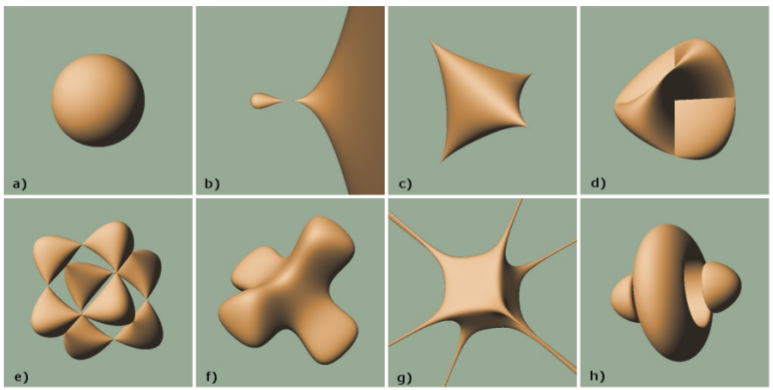
\includegraphics[scale=0.5]{images/florez6.png}
	\caption{Superficies usadas para comparar distintos métodos basados en intervalos para realizar Ray Tracing en superficies implícitas. a) Esfera. b) Superficie{ \em gota}. c) Kusner-Schmitt. d) Crosscap. e) Superficie Chubs. f) Modelo K3 McMullen g) Cubo astado. h) Toro Gumdrop.}
	\label{florez49}
\end{figure}

Como vemos en los resultados que extrae \cite{Florez08}, cinco han sido los métodos analizados: el algoritmo propuesto por Mitchell, el método de Newton basado en intervalos, el método de Newton usando el operador de Alefeld-Hansen, el algoritmo MRFro y un algoritmo que combina las condiciones del MRFro y las del método de Newton basado en intervalos.

\begin{remark}
Los resultados presentados por \cite{Florez08} se basan en imágenes de 300x300 píxeles de resolución  y fueron renderizadas en un ordenador con un procesador Pentium 4.
\end{remark}

\begin{figure}[h]
	\centering
	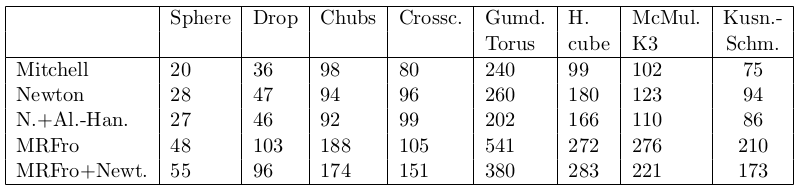
\includegraphics[scale=0.5]{images/florez7.png}
	\caption{Comparación de diferentes métodos.}
	\label{florez41}
\end{figure}

Obviamente los resultados son mejores para la esfera en todos los métodos y peores para una superficie compleja como el toro Gumdrop. El algoritmo de Mitchell muestra una mejor eficiencia para una superficie tan sencilla como es la esfera, pero cuando la complicación va aumentando el mejor método es el de Newton+AH. Además el método de Newton también mejora relativamente la velocidad, pero no lo suficiente. Esto nos indica dos cosas:
\begin{itemize}
\item Las comprobaciones extra que se necesitan en el operador de Alefeld-Jansen se compensa con la mejor convergencia en superficies complejas.
\item En el caso de superficies simples, como la esfera, es mejor aplicar métodos simples como el de Mitchell.
\end{itemize}

El algoritmo MRFro es el más lento en todos y esto es debido a que no toma información extra de la superficie como puede ser la derivada. Cuando se añade información extra, como la subdivisión de Newton, el algoritmo mejora su eficiencia en superficies complejas pero no para superficies simples.

La imagen \ref{florez410} nos muestra gráficamente los resultados de la tabla \ref{florez41}.  Las superficies fueron intencionalmente ordenadas de menos a más computacionalmente costosa.  Esto indica que la complejidad se incrementa de izquierda a derecha. Además un mayor tiempo indica menor eficiencia y viceversa.

Los algoritmos de Mitchell, Newton y Alefeld-Hansen tiene una eficiencia casi lineal cuando la complejidad crece. Además, la eficiencia es parecida en estos tres métodos que usan la derivada como fuente de información.

Por otro lado, el hecho de que tengan una eficiencia tan parecida nos hace darnos cuenta de que podemos usar operaciones con intervalos en todo el proceso sin afectar al tiempo de computación.

\begin{figure}[h]
	\centering
	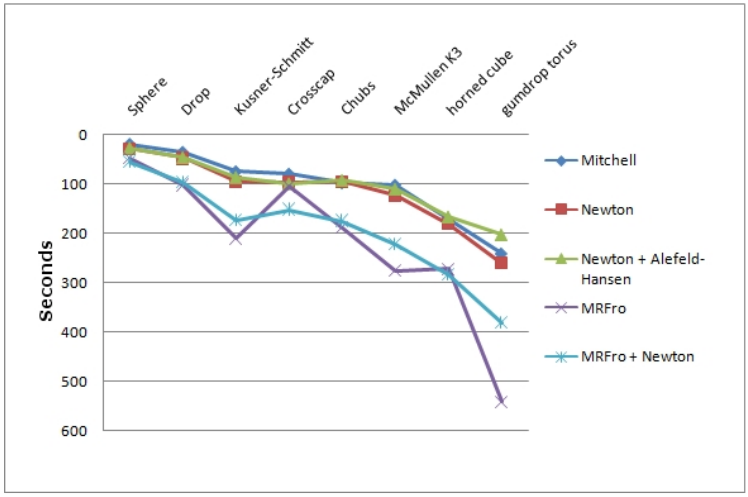
\includegraphics[scale=0.5]{images/florez8.png}
	\caption{Resultados de la comparación de diferentes métodos de Ray Tracing para las superficies analizadas. Las diferencias en calidad de renderización no son apreciables entre los métodos.}
	\label{florez410}
\end{figure}

\subsection{Otras aproximaciones destacables}

\subsubsection{Métodos basados en constantes de Lipschitz}

Dada una función implícita $h(t)$, si existe una constante positiva $L$ tal que para cualesquiera valores $t_1$ y $t_2$ se verifica
\begin{equation}
|h(t_1) - h(t_2)| < L |t_1 - t_2|,
\nonumber
\end{equation}
entonces se dice que $H$ satisface la condición de Lipschitz y $L$ se conoce por el nombre de constante de Lipschitz. Si $t_1$ se encuentra relativamente cerca de $t_2$, entonces
\begin{equation}
\frac{|h(t_1) - h(t_2)|}{|t_1 - t_2|} < L
\nonumber
\end{equation}
representa la derivada de la función $h$. En tal caso $L$ mide la variación de la función entre $t_1$ y $t_2$.

El método de las superficies L-G \cite{Kalra89} se basa en las constantes de Lipschitz para desarrollar un método eficaz y de confianza de Ray Tracing en funciones implícitas. Este método trabaja con dos pasos:
\begin{enumerate}
\item Se crea una estructura octal para la función implícita $f(x)$ con $x \in \mathbb{R}^3$ y y para la que existe una constante de Lipschitz $L$. Sea $x_0$ el centro de uno de los cubos y $d$ la distancia entre éste y cualquiera de los vértices, si $|f(x_0)| > Ld$ entonces podemos descartar el cubo. De otro modo el cubo se subdivide en otros ocho cubos nuevos. La mayoría de cubos se aceptará o rechazará sin problema, pero puede haber casos conflictivos como los que se muestran en la figura \ref{florez411}.
\begin{figure}[h]
	\centering
	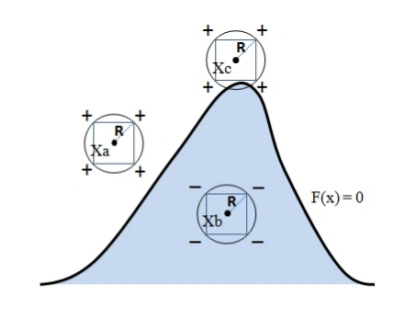
\includegraphics[scale=0.5]{images/florez9.png}
	\caption{Esferas con centro en $x_a$ y $x_b$ no intersecan a la superficie. Mientras que la esfera con centro en $x_c$ puede que sí la interseque.}
	\label{florez411}
\end{figure}

\item Se realiza Ray Tracing sobre la superficie usando la estructura creada en el primer paso. Si ahora consideramos la función intersección $g(t)$ con constante de Lipschitz $G$. Sean $t_1$ y $t_2$ los puntos de entrada de $g$ en un octal, entonces $t_m = \frac{t_1 + t_2}{2}$ y $d = \frac{t_2 - t_1}{2}$. Si $|g(t_m)| > Gd$ entonces existe una única raíz entre $t_1$ y $t_2$. 
\end{enumerate}

El algoritmo sería el que sigue:
\begin{verbatim}
Lipschitz(t_1,t_2):
   Compute G for t_1, t_2
   t_m = midpoint(t_1,t_2)
   d = (t_2 - t_1)/2
   If(abs(t_m) > G*d)
      If(F(t_1)*F(t_2) < 0)
         Compute using Newton
      Else
         There's no intersection
   Else
      Lipschitz(t_1,t_m)
      Lipschitz(t_m,t_2)
\end{verbatim}

Otro método basado en constantes de Lipschitz es el Sphere Tracing\cite{Hart96}. Este método es similar al de las superficies L-G pero usa cotas de Lipschitz en lugar de constantes de Lipschitz. Una cota de Lipschitz es cualquier constante que satisface la condición de Lipschitz, pero no necesariamente la más pequeña. En este método, debemos primero encontrar una cota de Lipschitz para una determinada función según qué distancia consideremos.

\subsubsection{Aritmética afín}

De Cusatis et al.\cite{Cusatis99} introdujeron el uso de aritmética afín al Ray Casting de superficies implícitas. La Aritmética de Intervalos puede generar una sobre estimación en algunas operaciones con intervalos. La Arimética afín se propuso para controlar  esta sobrestimación ya que la aproximación se realiza sobre un paralelogamo, véase \ref{florez413}. La Aritmética afín converge cuadráticamente mientras que la bisección usando Aritmética de Intervalos lo hace de forma lineal.
\begin{figure}[h]
	\centering
	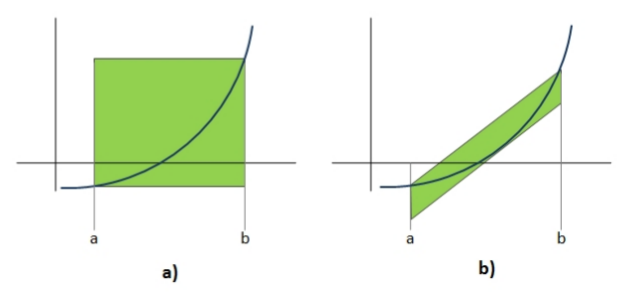
\includegraphics[scale=0.5]{images/florez10.png}
	\caption{Aproximación de una función en un intervalo $[a,b]$. a) Usando Aritmética de Intervalos. b) Usando Aritmética afín.}
	\label{florez413}
\end{figure}

En la Aritmética afín una cantidad $x$ se define mediante la forma afín
\begin{equation}
\hat{x} = x_0 + x_1 \epsilon_1 + \dots + x_n \epsilon_n,
\nonumber
\end{equation}
la cual es un polinomio de grado uno. Los elementos $\epsilon_i$ son desconocidos pero sabemos que oscilan en el intervalo $[-1,1]$. Éstos pueden contribuir a la incertidumbre de dos o más cantidades. Esto indica cierta dependencia subyacente entre las cantidades.

El esquema de este nuevo algoritmo es básicamente el mismo que el que describe este mismo concepto en la Aritmética de Intervalos. La diferencia es qué librería ha de usarse para el cálculo de las extensiones unidas. Como pasa en la Aritmética de Intervalos, las operaciones de aritmética básicas y funciones pueden ser extendidas a formas afines que sean manejables\cite{Stolfi97}.

Sin embargo, las mejoras introducidas por el uso de Aritmética afín van en detrimento del algoritmo básico propuesto por Mitchell\cite{Cusatis99}, pero no en detrimento de en un método más veloz como el de Newton con intervalos. Además, ha sido probado que la Aritmética afín es un caso especial de la forma centrada de la Aritmética de Intervalos\cite{Gavriliu05}.

\section{Conclusiones}

En este capítulo hemos hecho una introducción de diferentes aplicaciones de la Aritmética de Intervalos en la creación de estructuras de subdivisión y también en la creación de test de intersección de Ray Tracing en superficies implícitas. La Aritmética de Intervalos nos proporciona una manera sencilla de comprobar los tres ejes de un cubo para saber si interseca a la superficie. Esta técnica puede ser mejorada mediante el estudio de la superficie para realizar más subdivisiones en secciones críticas de ésta.

Además, también hemos presentado diferentes técnicas para realizar test de intersección entre rayos y superficies implícitas. La mayoría de métodos para los test de intersección están destinados a trabajar con Aritmética de Intervalos, la cual remplaza las operaciones sobre número reales por operaciones sobre intervalos.

Hay diferentes aproximaciones, por ejemplo, las basadas en derivadas y otras que crean ciertas condiciones para mejorar el proceso de bisección. Aunque  el uso de derivadas mejora la eficiencia, puede que ésta no sea fácil de obtener para algunos tipos de superficies implícitas. Dimos también un rápido vistazo a la comparación de distintos métodos para saber su comportamiento y eficiencia ante las mismas superficies con distinta complejidad y vimos que en superficies sencillas son máś eficientes algoritmos sencillos y en superficies complejas es más eficaz el uso de algoritmos algo más complejos debido a que suelen presentar convergencia de orden cuadrático frente a la lineal de los más simples, lo que compensa las comprobaciones extras que deben realizarse.

Finalmente también vimos como hay otra serie de técnicas que no usan Aritmética de Intervalos como las basadas en constantes de Lipschitz o en Aritmética afín. Aunque su perdida de generalidad les hace menos atractivas y, por tanto, su uso está muy poco popularizado.